\chapter{技术路线、现有方法分析及背景支持}

\section{技术路线分析}

事实上,承上一章所述之背景,设计工作和艺术创作虽然强烈依赖作者的感受力和创造性,但是在某些环境下也是重复的脑力活动。例如在游戏美术、电影场景绘画、高概念电影故事创作以及网络小说的写作等工作中,创作常常符合某种模式,其重复的模式非常多。在此模型下,艺术创作可以抽象为一个制作或者生成过程,如方程\eqref{eq:gene-art}所示。 

\begin{equation}\label{eq:gene-art}
ArtWork= Generator(f_0, f_1, f_2, \cdots, f_N, r_{x \sim p})
\end{equation} 

但是由于传统机器学习的两个特点,使得艺术生成并不适用传统机器学习的方法,第一是:其输出是一个序列性的而非特点长度的标签(Label)或者回归预测值; 第二是: 艺术的输入特征难以确定, 其输入也是一个复杂的序列过程。这两个因素使得计算机进行自动艺术创作在长时间内仍然依赖于人类编写规则,使得计算机艺术创作不能广泛得适用于更加通用的场景。 

而深度学习在特征自动学习(Representation Learning )和序列数据特征的提取中均具有良好的效果,所以很多科研工作者开始使用深度学习相关的方法来尝试计算机自动生成艺术作品。 

色彩方案设计是在设计领域中普遍的一个工作方式。作为一个设计师,在每个项目中,选取合适的配色方案是一个重要的工作。在设计师设计的过程中,例如设计服饰,软装设计,建筑外观设计等,依据现有的环境特点,应用场景,目标用户,需要制定配色方案,然后将配色方案应用于整体方案上,有时配色方案还会应用到成套的产品中的各个子产品。由于自然语言理解与图像识别等领域目前都有了长足的进步,所以设计作品自动配色这个问题目前有可能使用神经网络和深度学习的内容进行自动化。 

而且,由于自然语言理解在最近几年取得的成果,其在语义理解方面可以良好的应用于设计作品自动配色这样领域。目前,计算机辅助设计在这方面的方式是采用一张配色表,使用关键词进行配色,例如图 \ref{img:peise} 这种方式进行。 这种方式其实是计算机语言理解的时候的一种折中做法。 

\begin{figure}[htbp]
    \centering  % 学位论文规定图表皆水平居中于版心 在 zjuthesis.cls 搜「版心设置」
    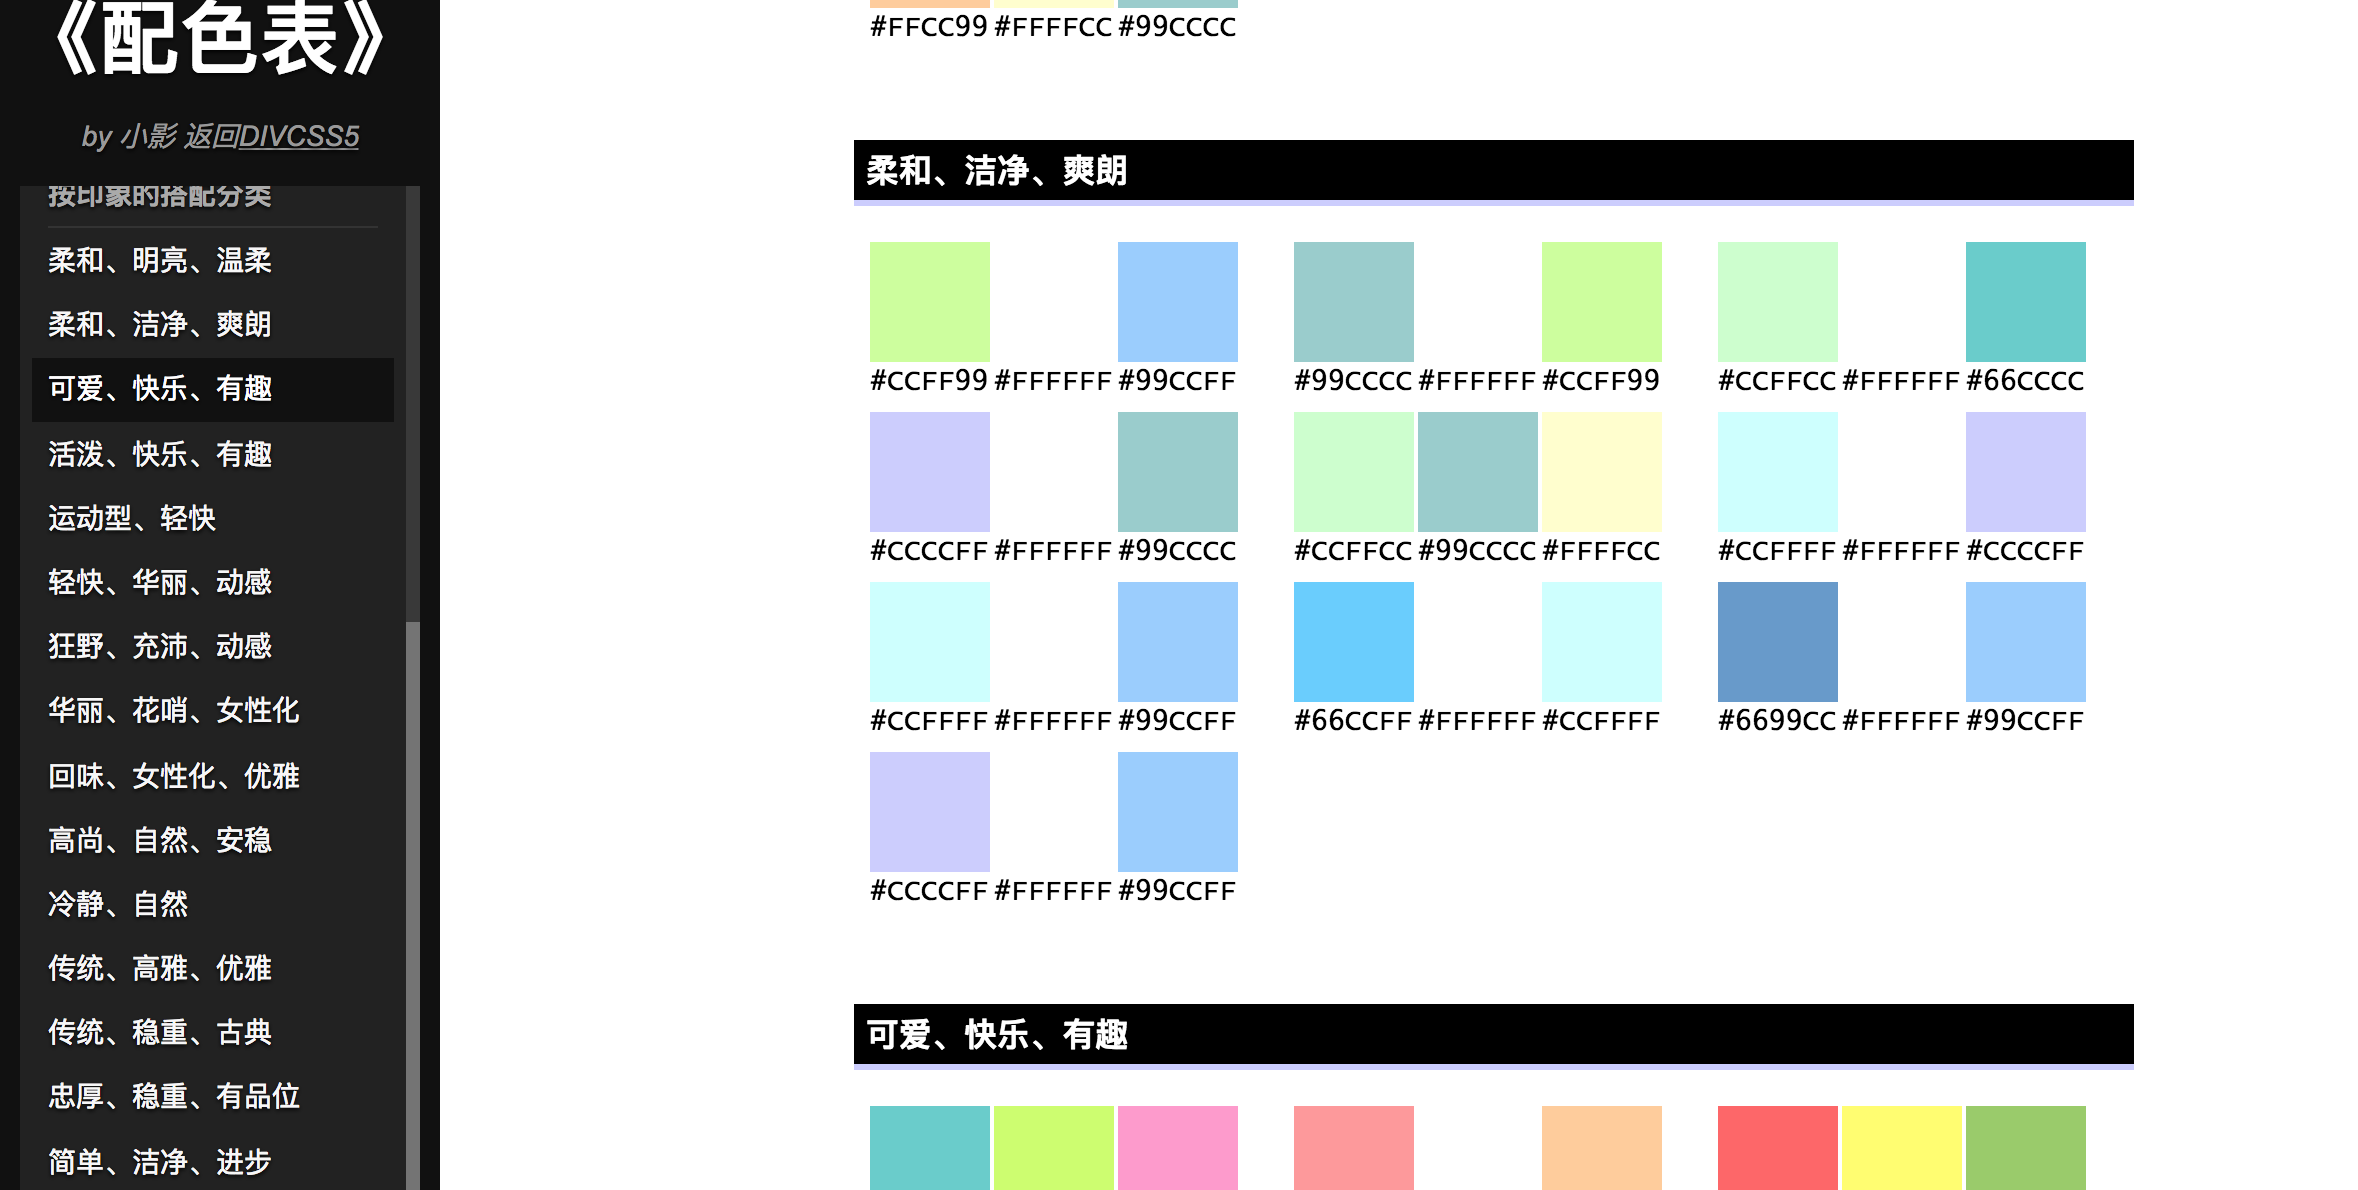
\includegraphics[width = .55\linewidth]{data/chapter-2/peisebiao.png} % 设定图片宽度相对于版心宽度,图片文件资源名
    \caption{设计师使用配色表进行配色} % 图的题注
    \label{img:peise} % 与 autoref 关联,设定交叉引用和显示「图x.x」
\end{figure}

这种方式存在两个问题:第一, 有限的词汇其实不能表达丰富的含义,设计作品的应用涵盖生活的方方面面, 其需要表达的语义丰富性是远远高于有限的这些单词的; 第二,单个词汇与整体意向组织不具备线性叠加的关系。 即, 设计师要设计出一个“温柔的春天”这样意境的设计作品, 其颜色不能是先选择“温柔”, 再选择“春天”, 而是需要再次进行加工。 将这两种的意向进行重叠。 而这种加工是目前的配色表不能完成的。 

因此, 本课题希望基于目前的自然语言理解的技术与图像自动化处理的方式, 实现从作者的直接描述到自动产生配色图的自动化转化。 例如, 一个设计师接到了室内软装设计的需求, 甲方的需求是\textbf{“洋溢着春天的感觉, 要很温柔, 然后要像有小孩在草坪上奔跑一样”}, 本课题要实现的基于语义识别的自动配色系统,只需要将这句话\textbf{“洋溢着春天的感觉, 要很温柔, 然后要像有小孩在草坪上奔跑一样”},输入到系统中,就会自动匹配色彩方案,并且可以为直接其线稿进行上色,可以方便的预览,把握整体风格,参考及其方便,甚至批量生成预览图像,为客户展示和预览也节省大量时间。

基于之上的分析,本课题研究一种例如深度学习与表示学习的方式,在此基础上实现从语言理解到色彩搭配的自动转化。之后,本课题在真实数据库上进行了实验,本模型确实能够实现良好的自动化转化,证明了该模型的有效性。 


\section{国内外研究现状}

因为本研究课题是机器学习、自然语言处理和图像合成的交叉领域, 本小节主要从以下三方面进行国内外现状的分析: 

\begin{enumerate}

	\item 自动图像合成
	\item 表示学习 (Representation Learning)
	\item 序列化生成 
	
\end{enumerate}


\subsection{计算机自动图像生成} 实现计算机自动图像生成或自动色彩搭配,目前涉及到的方法如下: 

\begin{itemize}

	\item 查表法
	\item 马尔可夫链
	\item 机器学习与人工智能方法
	\item 原细胞有限自动机
	\item 基于规则的算法 [Wiggins(1991), Nierhaus(2009)]
	
\end{itemize}

%除使用以上方法, 目前仍有人工定义负责算法进行音乐的自动合成, 例如Wiggins(1991), Nierhaus(2009)。 

使用机器学习与人工智能方法主要分为两个类型, 一是监督式的(Supervised), 希望给计算机一定的监督样本(Samples), 使得计算机能够拟合一个函数, 使得该函数能够拟合训练数据到已知样本标签的映射如等式 \eqref{eq:map}

\begin{equation}\label{eq:map}
function(x) \rightarrow y
\end{equation}

监督式的学习方式在图像生成领域应用不多, 主要使用因为该种方式主要应用在问题结果确定已知并且有限的情况下, 即 其目标函数的$y in \mathbf{R}^n$ 且 $|y| <= N$ 。 但是, 在图像生成领域,目标函数的结果大家的期望并不是从已知的范围内选择一些出来,而是希望能够自动创作。 

所以目前机器学习方式主要采用\textbf{非监督学习}的方式进行图像生成。 非监督的学习方式主要通过从已知的信息中, 获得不同类型的信息、数据的隐含关系, 例如图 \ref{img:unsupervised}。 

\begin{figure}[htbp]
    \centering 
    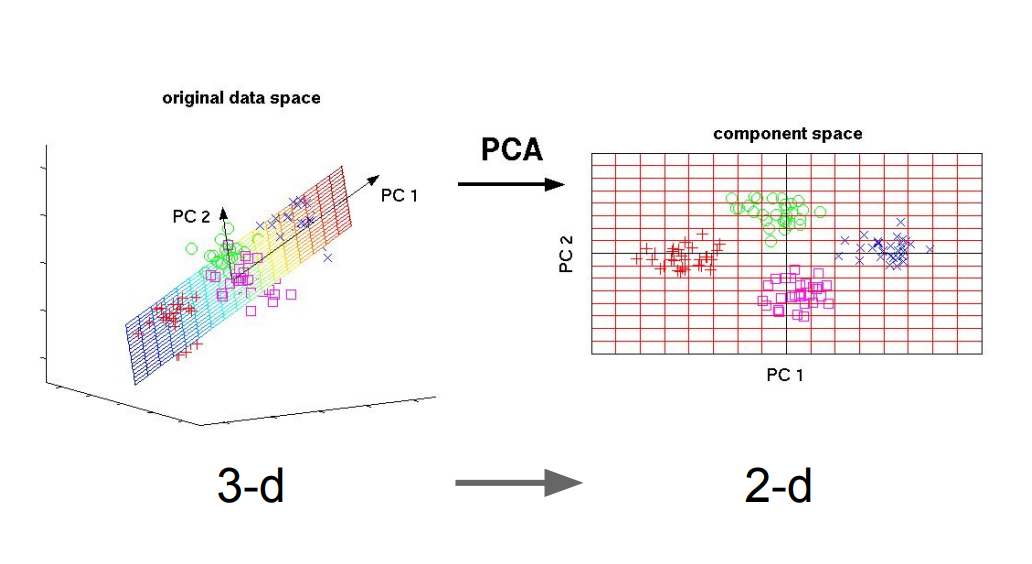
\includegraphics[width = .55\linewidth]{data/chapter-2/unsupervised.png} 
    \caption{非监督式学习主要用来找到影藏的关系} 
    \label{img:unsupervised} 
\end{figure}

而基于非监督式的学习, 提出的Autoencoder 自编码模型可以在缺少某些信息的情况下, 对图像进行重建。 例如图 \ref{img:autoencoder} 所示。

\begin{figure}[htbp]
    \centering  
    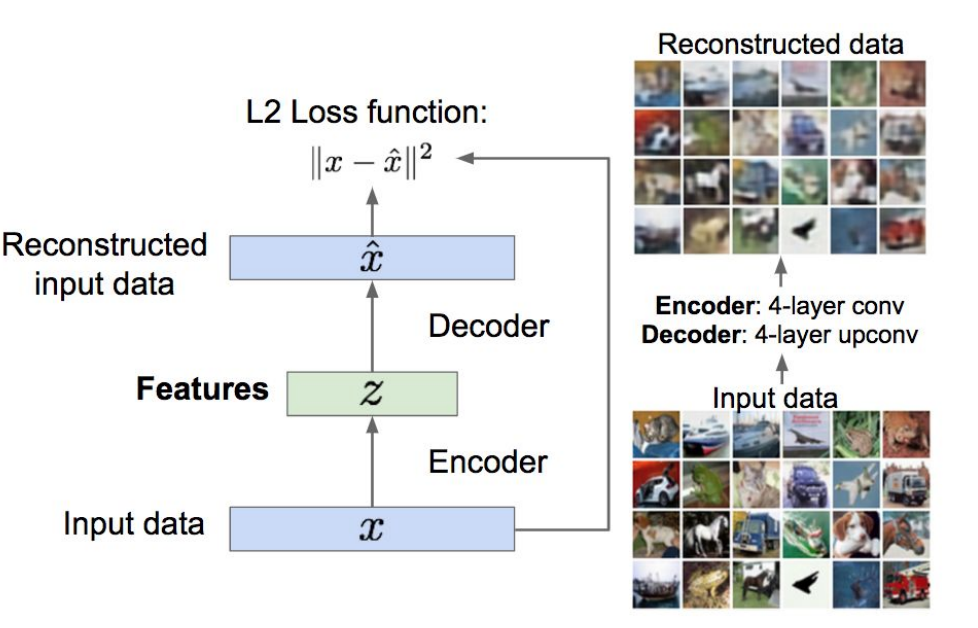
\includegraphics[width = .55\linewidth]{data/chapter-2/autoencoder.png} 
    \caption{自编码模型可以从缺少的信息中重建图片} 
    \label{img:autoencoder} 
\end{figure}

由于重建信息的成功, 如图 \ref{img:autoencoder}, 科研人员考虑如何通过已知的数据, 获得其潜在的数据概率分布, 从而可以不依靠部分信息而对全部的信息进行重建, 以重建其具备与源数据源具有同样数据分布的数据。 

\begin{figure}[htbp]
    \centering  
    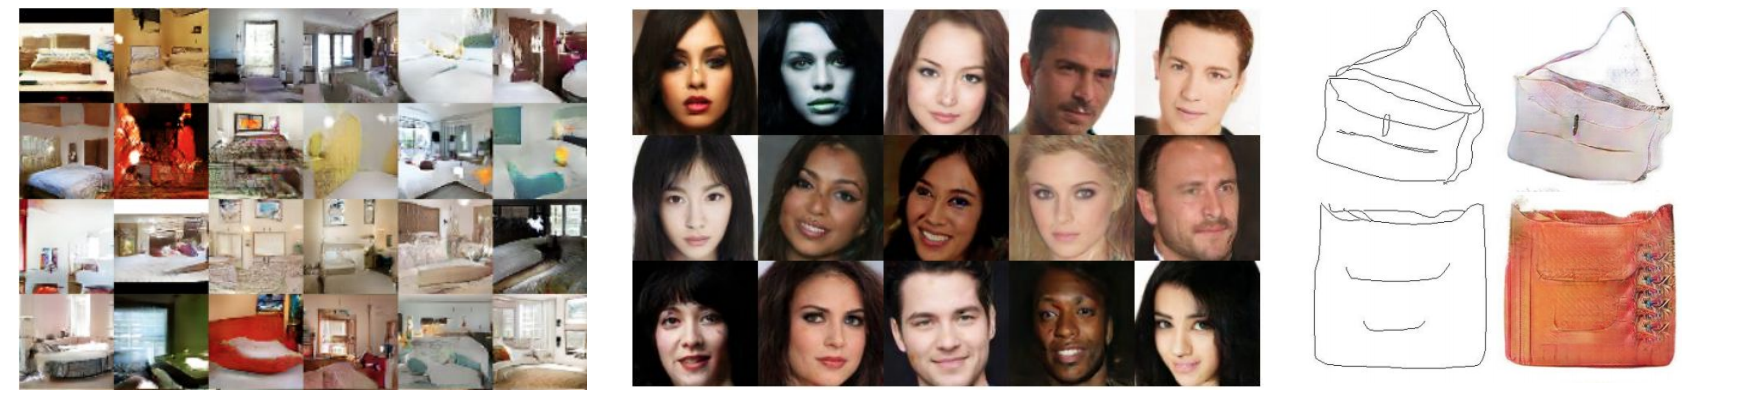
\includegraphics[width = .55\linewidth]{data/chapter-2/gene.png} 
    \caption{生成模型可以直接生成新的信息而不基于输入的部分信息} 
    \label{img:gene} 
\end{figure}

要完成此任务, 目前主流的使用PixelRNN/CNN, GAN,马尔科夫连, 以及模仿学习(Imitation Learning), 这些模型都可以模型训练之后, 不需要输入部分“初始信息”, 而直接获得新的符合原来数据分布的新数据, 例如图 \ref{img:gene} 所示, 模型可以随机的产生室内的图片, 人像, 以及自动为线稿配色。  



\subparagraph{计算机生成图像——GAN} 随着理论研究的发展,计算机艺术辅助工具也有了新的突破,通过对抗神经网络算法(Generative adversarial networks - GAN),能够自动生产图片。\cite{radford2015unsupervised},GAN由判别器和生成器实现,判别器对照相机拍的照片和生成器生成的图像进行分类,而生成器从随机噪声中生成尽可能以假乱真的图像,判别器和生成器相互对抗,最后生成判别器无法判别的图像。这种模型,可以生成现实风格的图像,也可以用于将马赛克还原为清晰的照片。使用GAN可以根据文字生成图片,如图~\ref{figure:GAN}。\cite{goodfellow2014generative} \cite{mcaleergenerative}

\begin{figure}[!htbp]
\centering

\includegraphics[width=\linewidth,keepaspectratio]{data/chapter-1/gan.jpeg}
\caption{GAN从文字生成真实的图片}
\label{figure:GAN}
\end{figure}

图~\ref{figure:GAN}中显示基于GAN可以根据一句话,例如“小鸟,胸部和冠羽是粉红色的,黑色的一级和次级飞羽”就可以生成类似照片的图片。使用“胸部和冠羽是粉红色的鸟”和“黑色飞羽的鸟”的照片作为真实照片进行训练,生成器生成尽可能以假乱真的图像,判别器对真实照片和生成器生成的图像进行分类,相互对抗,最后生成判别器无法判别的图像。于是生成器就可以生成满足“小鸟,胸部和冠羽是粉红色的,黑色的一级和次级飞羽”这句话的图片。GAN生成的图片非常真实,但是每每面对新的一句话,它就需要大量的图片和较长的时间训练GAN模型。

\subparagraph{自动配色的探索}pixel2pixel相关的工作中也有关于配色选取的工作。colormind使用pix2pix的方式从输入照片提取生成色彩方案。\cite{pix2pix2016}\cite{chen2015improved}与此同时也有研究者研究通过大数据探讨关于配色的问题,多伦多大学的Peter O'Donovan等人通过color.adobe.com、www.coluorlover.com等配色网站上用户对各类配色的打分数据,使用机器学习的方式学习为色彩的和谐程度打分。\cite{O'Donovan:2011:CCL:2010324.1964958}

\begin{figure}[!htbp]
\centering
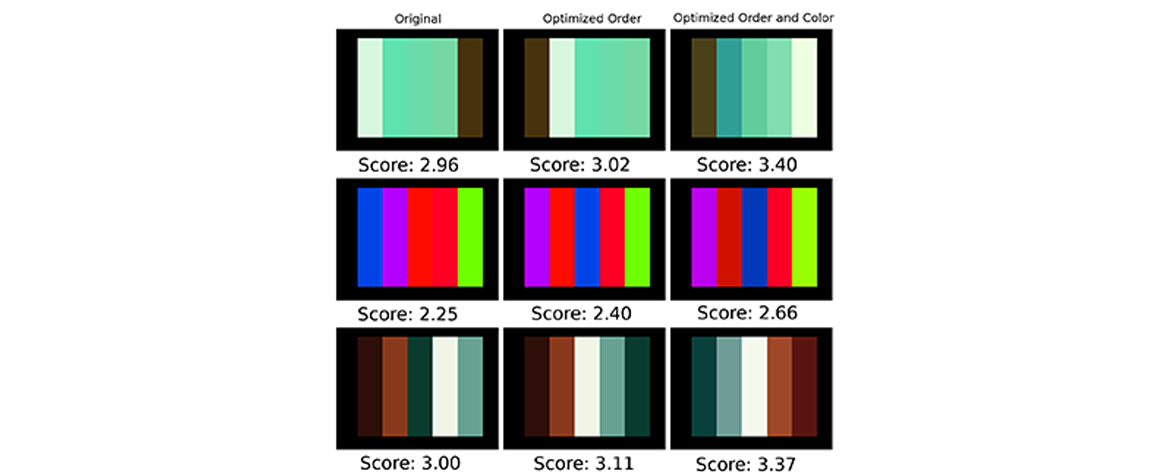
\includegraphics[width=\linewidth,keepaspectratio]{data/chapter-1/Color Compatibility.png}
\caption{从大量图片中学习色彩和谐程度}
\label{figure:Color Compatibility}
\end{figure}


\subparagraph{自动上色}

pixel2pixel探讨了更多基于对抗神经网络的,从图像生成图像的应用。在这一系列的相关工作中,包括能够为黑白照片自动上现实的合理的颜色,也可以为轮廓填充现实的合理颜色,以及从符号化的色块表达生成现实风格的图片,自动生成遮罩,自动替换照片中的人物。\cite{deng2010binary}

\begin{figure}[!htbp]
\centering
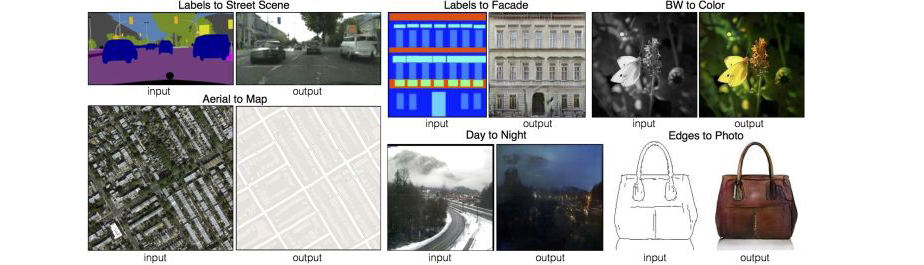
\includegraphics[width=\linewidth,keepaspectratio]{data/chapter-1/pix2pix.jpg}
\caption{pixel2pixel的若干应用}
\label{figure:Manga Colorization}
\end{figure}

有若干的项目都在讨论关于日本式漫画的自动上色问题,例如PaintsChainer和 Manga Colorization,如图~\ref{figure:Manga Colorization}。\cite{Qu:2006:MC:1141911.1142017} \cite{DBLP:journals/corr/ZhangJL17} 日式漫画风格较为统一,图形基本封闭,模式较为固定,并且对批量上色要求巨大。Manga Colorization能在标注颜色的情况下为二次元图片自动上色。PaintsChainer不局限于封闭的图形,并且自动完成上色与阴影模式,但其就效果而言,常常出现不可控的色块和理解错误的内容。

\begin{figure}[!htbp]
\centering
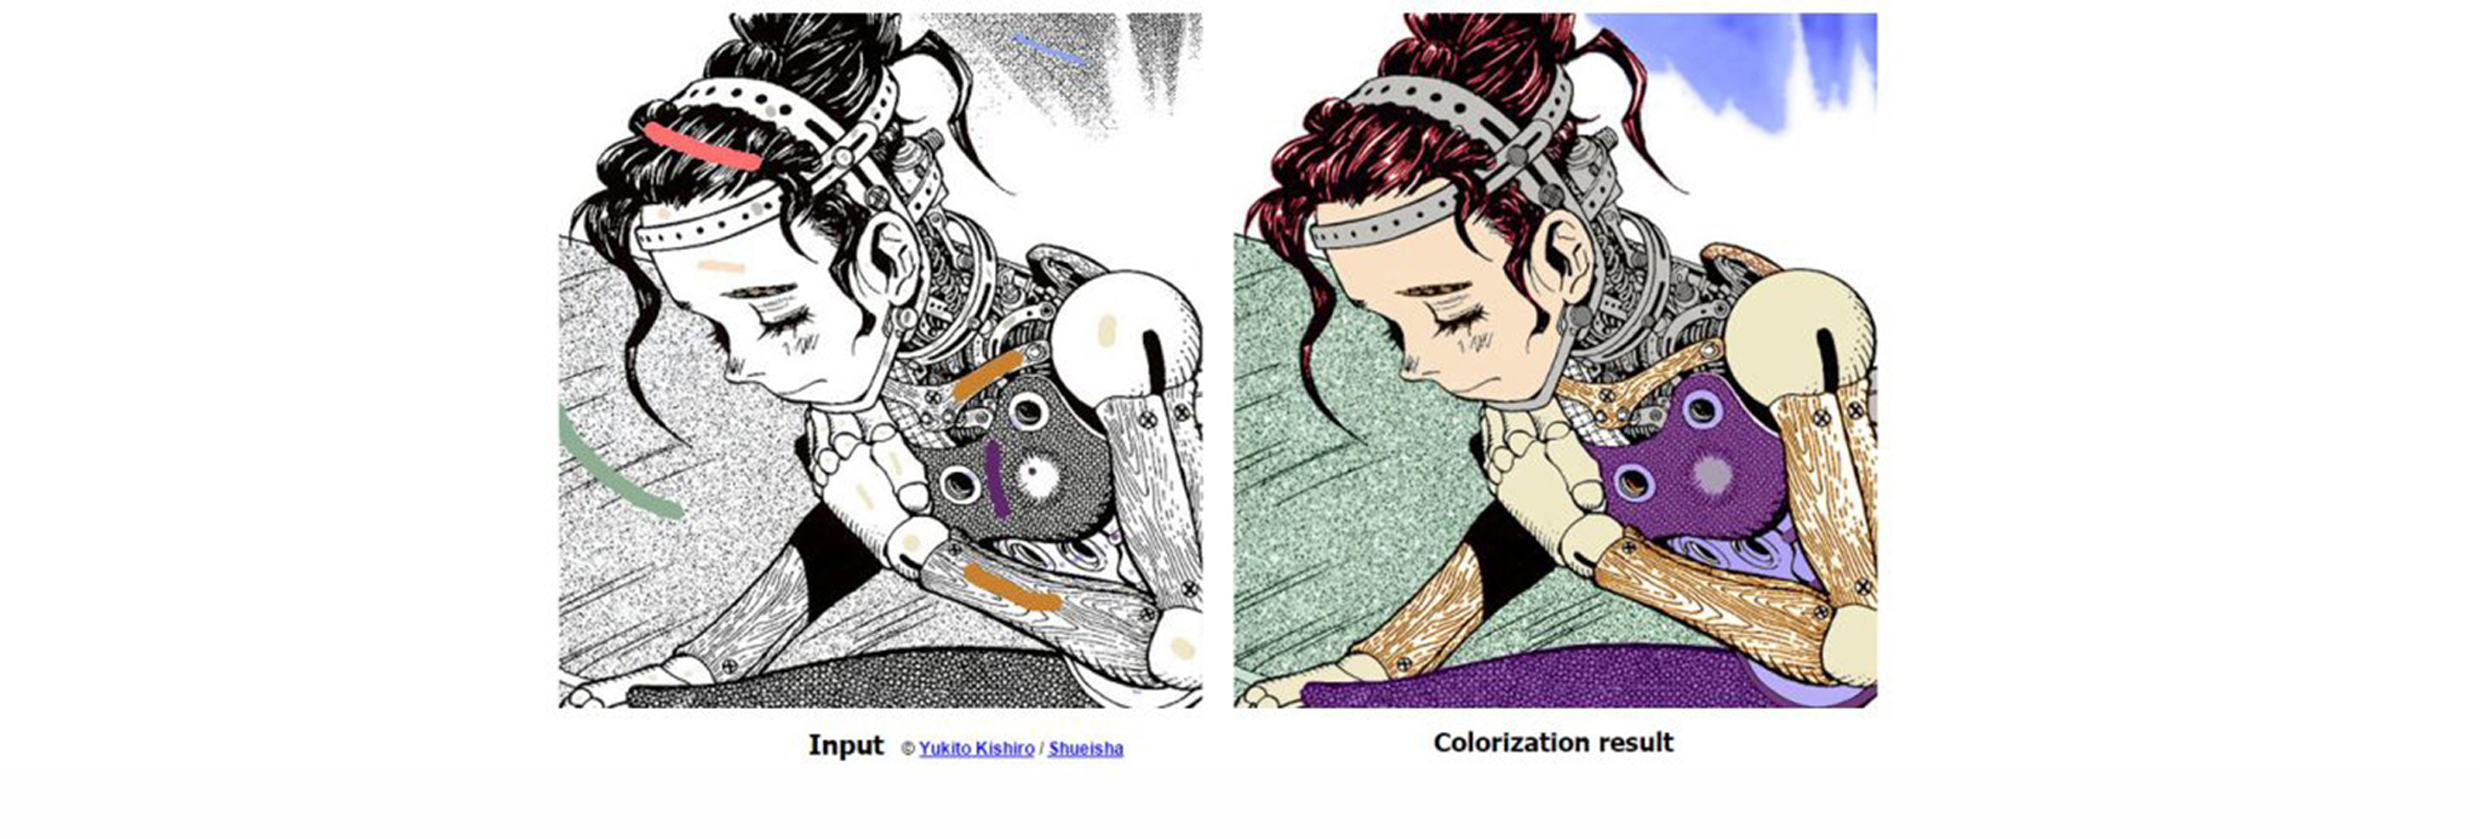
\includegraphics[width=\linewidth,keepaspectratio]{data/chapter-1/Manga.jpg}
\caption{Manga Colorization在标注颜色的情况下为二次元图片自动上色}
\label{figure:Manga Colorization}
\end{figure}

\subsection{表示学习与Embedding} 

表示学习是机器学习中重要的研究内容, 主要研究如何将数据有效的表示到计算机中。 其中, 最重要的的方式是如何通过一种方式使得新表现的数据形式能够保持其原始线性关系\cite{embedding}, 这种行为在计算机及数学中叫做embedding。Embedding是指,保持一种偏序关系,是的我们已知的某种关系也保持到新的向量空间中。 Embedding的具体定义如下:

$$ \forall x_{1},x_{2}\in X:x_{1}\leq x_{2}\Leftrightarrow F(x_{1})\leq F(x_{2}). $$


例如,之前人们对自然语言进行计算的时候, 使用的表示方式多是one-hot方法表示单词或者利用tf-idf等信息表示一句话。 但是这种表示并不能表征有效的表征句意。 Mikolov 等科学家使用的word2vec, 使得我们能够获得更加深层次的语义 \cite{DBLP:journals/corr/abs-1301-3781}。 由于word2vec保持了词汇意思的线性关系, 使得我们利用已知的单词获得新的,意思解决的单词变成了可能。 在Mikolov提出了Skip-Gram和CBOW等word Embedding的方法之后, 斯坦福大学NLP组提出的Glove,以及Salesforce提出的ContexVec \cite{DBLP:journals/corr/abs-1708-00107} 都获得更加良好的表现。 


\begin{figure}[htbp]
    \centering  
    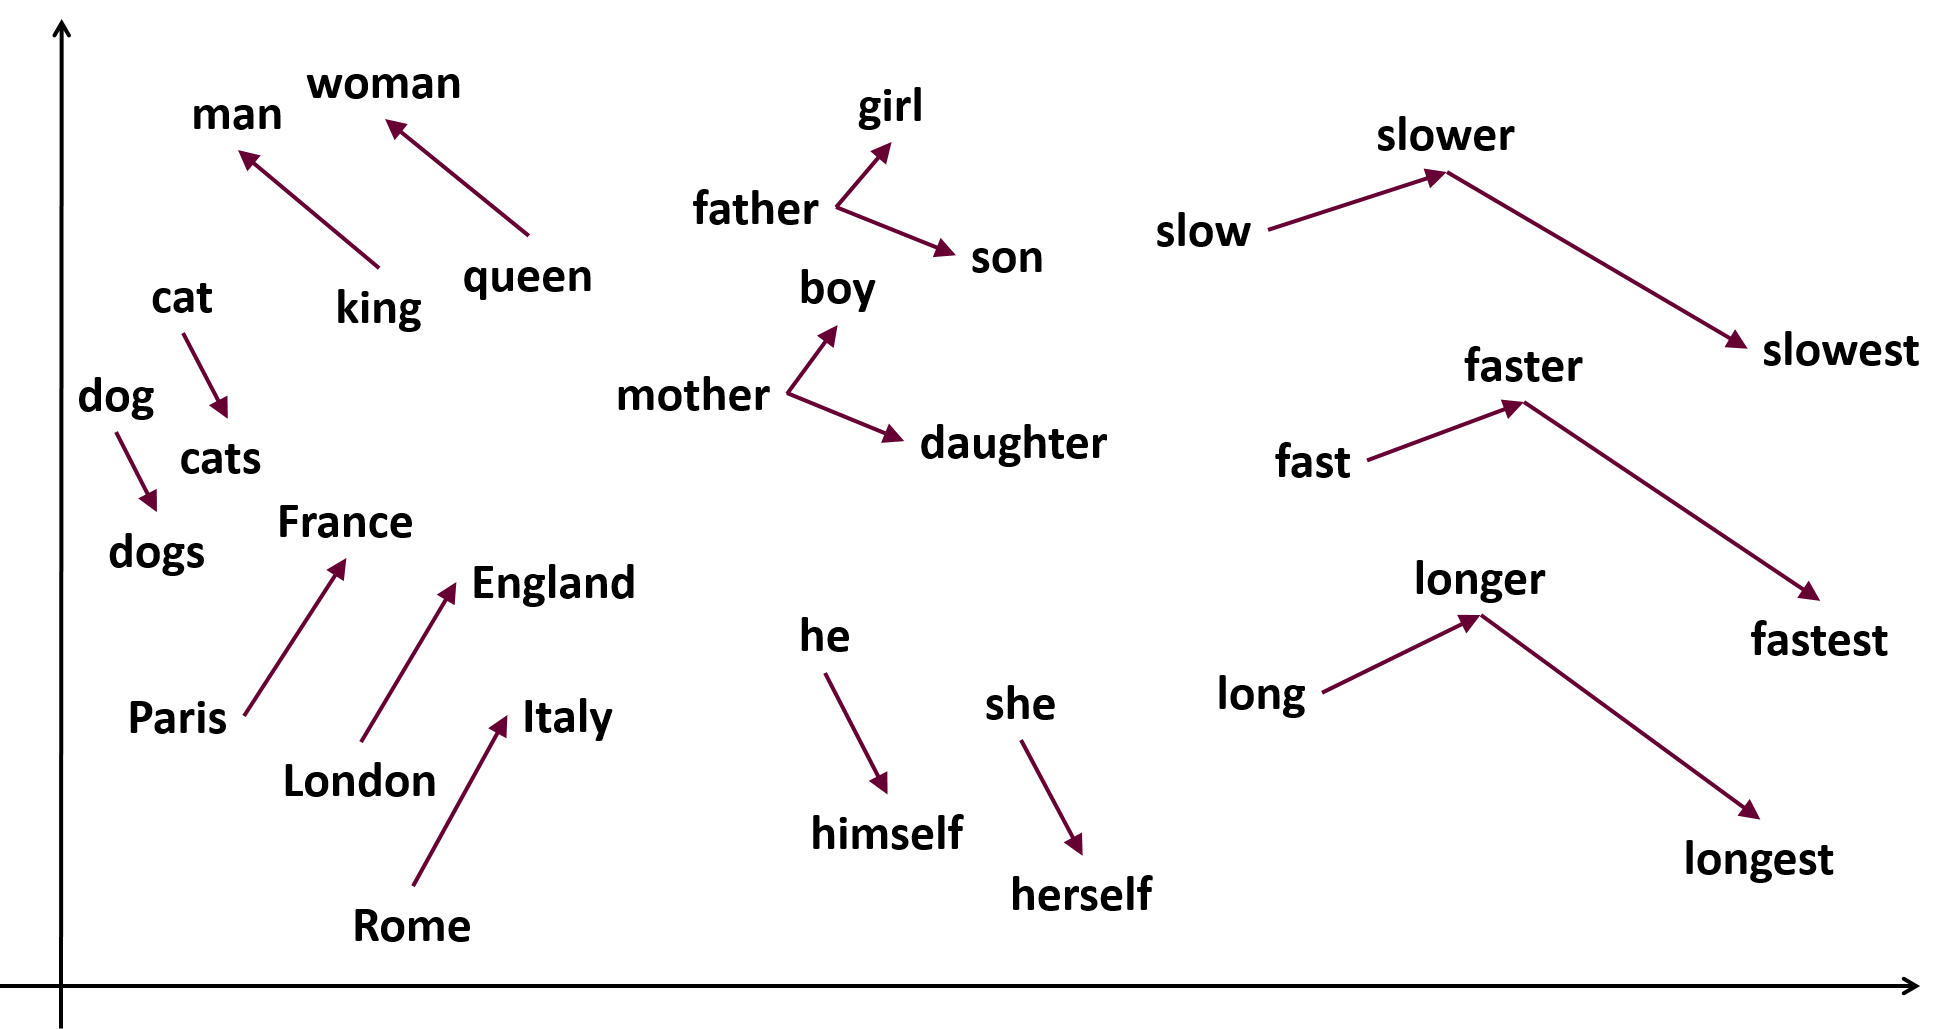
\includegraphics[width = .85\linewidth]{data/chapter-2/word2vec2.png} 
    \caption{Word Embedding 对单词词义的线性保持} 
    \label{word2vec} 
\end{figure}

\subsection{序列化生成:PixelRNN/CNN}

\begin{equation}\label{eq:pix}
p(x) = \prod_{i=n}^{n} p(x_i|x1, ..., x_{i-1})
\end{equation}

该模型基于一个信念网络(Belief network) \eqref{eq:pix}, 其中, $ p(x) $ 是某图像 $x$ 的似然分布, 而 $pr(x_i|x_1, ..., x_{i-1}$ 是某个像素的概率在给定该像素之前的所以像素分布之下的条件概率。 该信念网络希望通过网络模型获得其条件概率的最大分布。 要生成一个像素 pixel 需要获得上一个 pixel的值, 通过一个RNN或者CNN网络, 实现序列化的生成, 如图 \ref{img:pix-matrix} 所示。 

\begin{figure}[htbp]
    \centering 
    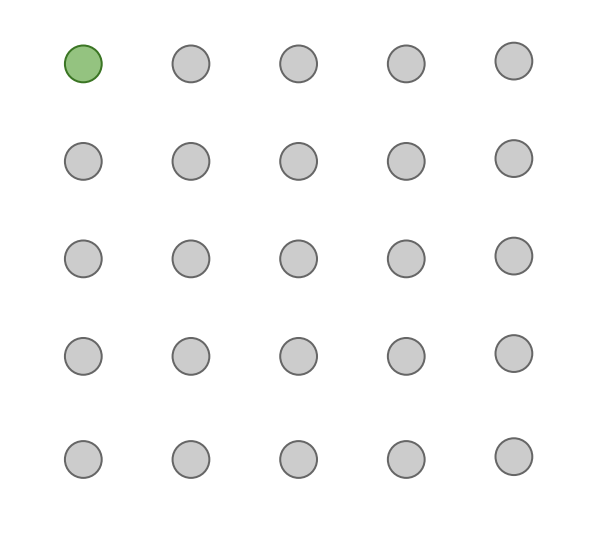
\includegraphics[width = .55\linewidth]{data/chapter-2/pixel_matrix.png} 
    \caption{pixel network 通过序列化的像素生成图像} 
    \label{img:pix-matrix} 
\end{figure}

依照此模型, 可以自动生成图像, 例如图 \ref{img:pix-example} 所示, 该模型在进行CFAIR10和ImageNet数据库的训练之后, 能够随机生成与之类似的图形. 

\begin{figure}[htbp]
    \centering  % 学位论文规定图表皆水平居中于版心 在 zjuthesis.cls 搜「版心设置」
    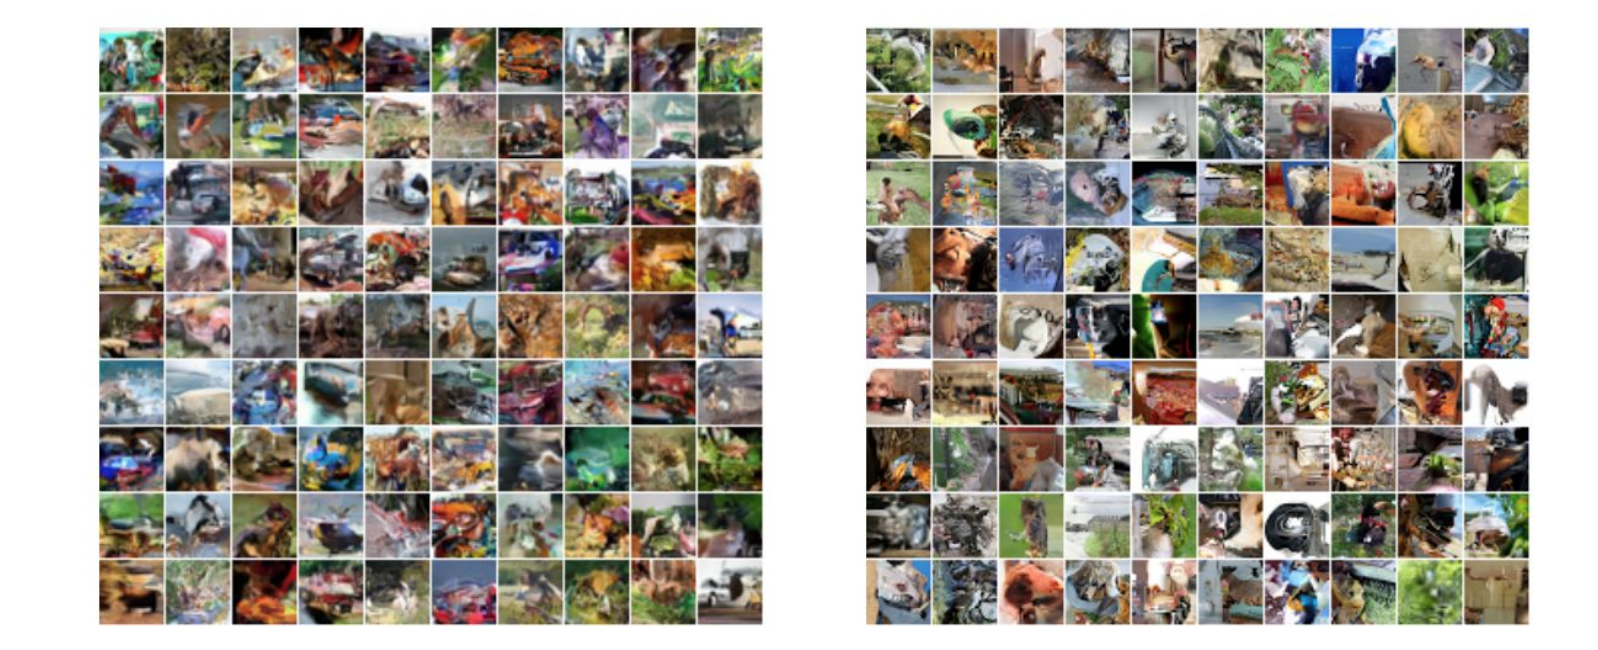
\includegraphics[width = .55\linewidth]{data/chapter-2/pixel_example.png} % 设定图片宽度相对于版心宽度,图片文件资源名
    \caption{pixel network 通过序列化的像素生成图像} % 图的题注
    \label{img:pix-example} % 与 autoref 关联,设定交叉引用和显示「图x.x」
\end{figure}




\section{数据库资源}

\subsection{艺术品交易数据库}

本文使用的数据库资源来自雅昌拍卖网艺术品交易数据库(auction.artron.net)。这是一个艺术品拍卖网站,数据库中关于艺术品以及艺术品交易的信息丰富,包括流通的艺术品的题目、图片、特征、作者、艺术品类别、交易价格、流通时间等等。我所用到的数据库中的信息包括两类如图~\ref{figure:数据库结构},一类是艺术品信息,另一类为艺术品相关的文章。

\begin{figure}[!htbp]
\centering
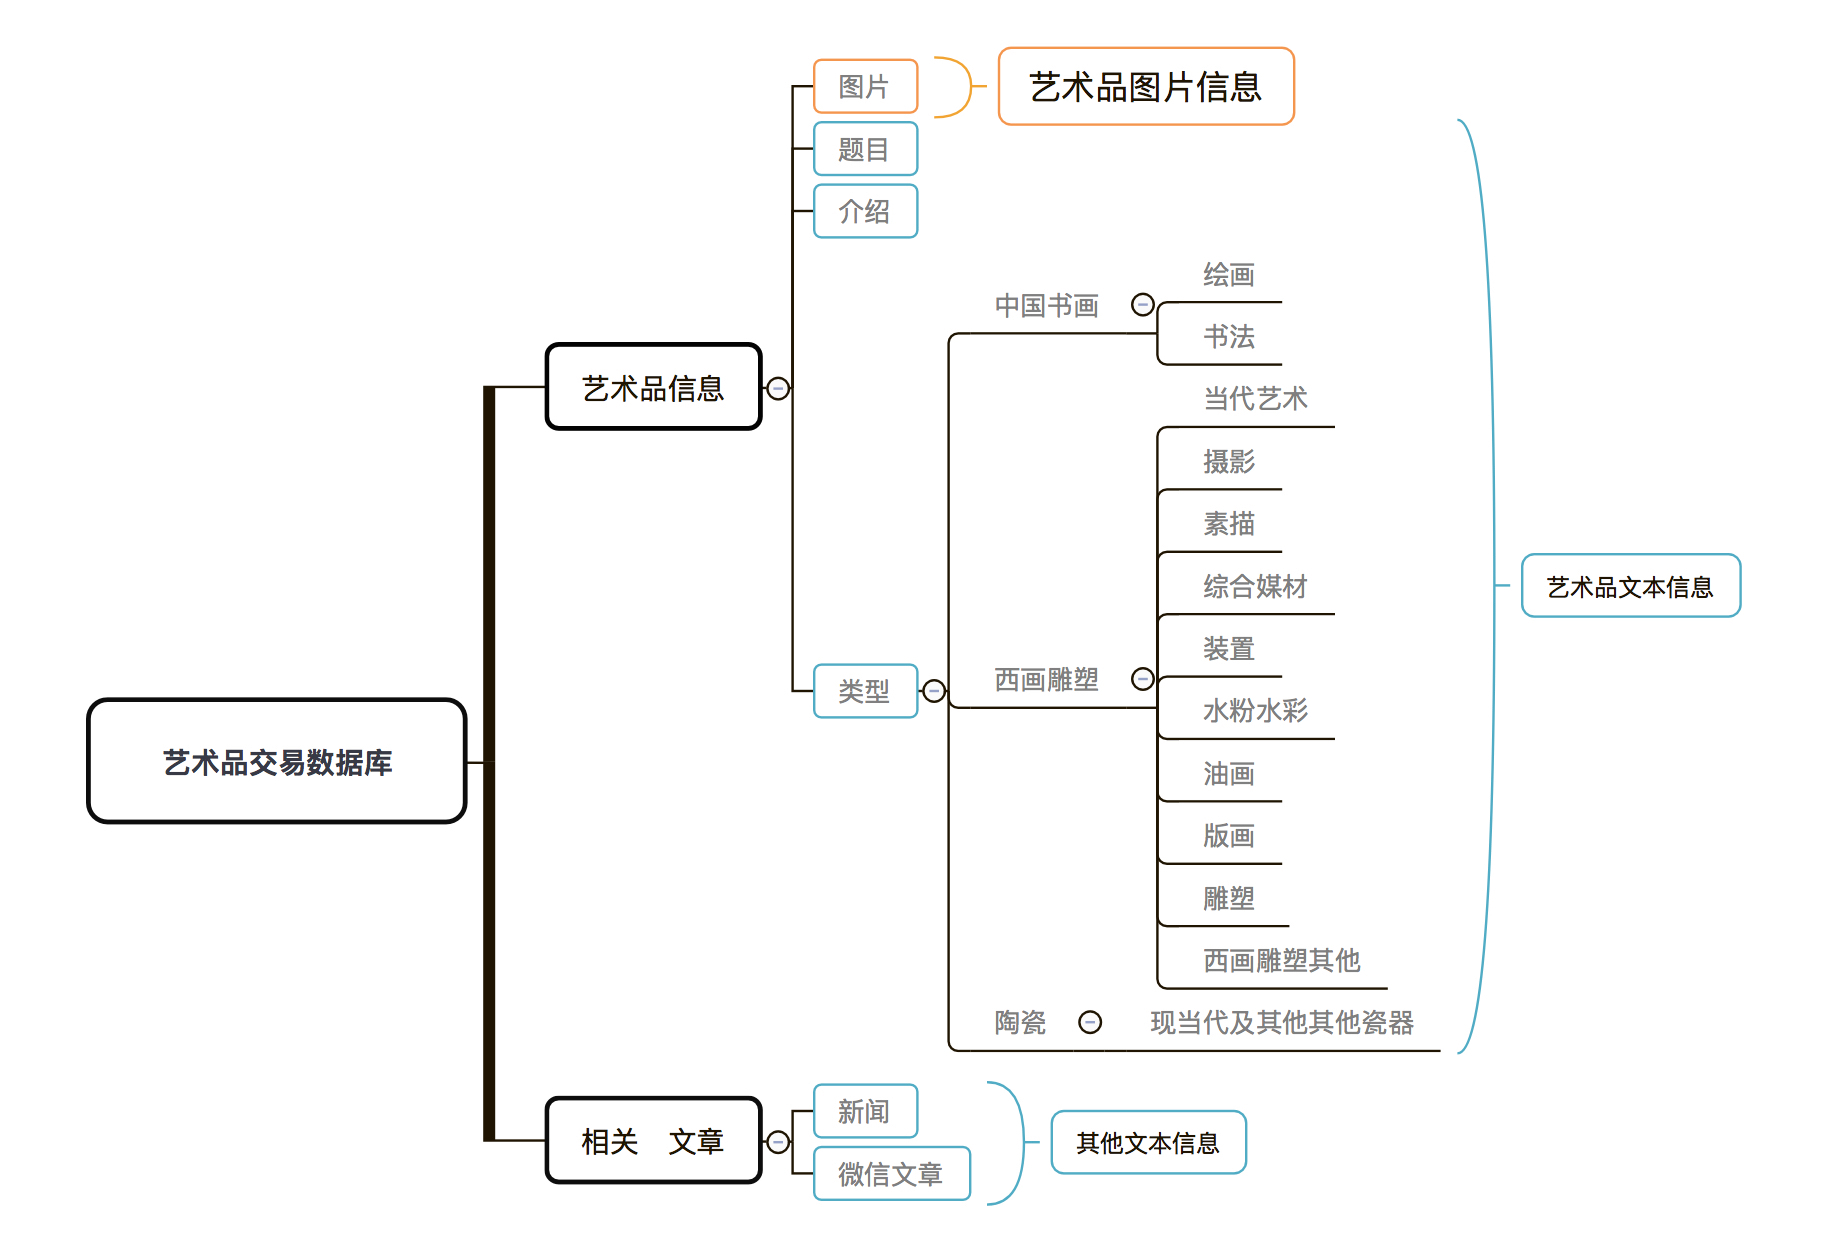
\includegraphics[width=\linewidth,keepaspectratio]{data/chapter-1/D02BCA18-F339-4988-9E23-E6C5E437BCCA.jpg}
\caption{数据库结构}
\label{figure:数据库结构}
\end{figure}

艺术品信息具体是指艺术品的题目、介绍,类型等文字描述(文本信息),以及艺术品的图片所在的url地址(可以下载到图像文件)。

每件艺术品都有对应的题目,艺术品的题目就是艺术品的名称,一般由艺术家命名,艺术品的名称和艺术品的内容常常是相匹配的。虽然也有一些情况艺术品的名称和内容表面上完全无关,但是艺术史上叫做“无题”的艺术品也何其之多,但是艺术品的题目作为艺术品的一部分,与艺术品的主题之间的关系紧密是无可辩驳的。

数据库中艺术品的类型分为中国书画、西画雕塑、陶瓷,在每个类型下再次细分。在中国书画下分为:绘画、书法。西画雕塑下分为:当代艺术、摄影、素描、综合媒材、装置、水粉水彩、油画、版画、雕塑、西画雕塑其它。陶瓷下分类为:现当代及其它瓷器。

数据库中艺术品的图片包括瓷器、雕塑等三维作品的照片和绘画、书法等二维作品的扫描件,由于数据库的数据缺失,极少量的艺术品并没有对应的艺术品的图片。

数据库中艺术品的介绍是艺术品交易时所附的艺术品介绍,内容包括并不限于对作者背景的介绍、该作品创作背景的介绍、作者风格的描述、作品风格和作品内容的描述等等,由于一些艺术品本身并没有对应的介绍文本以及数据库数据的缺失,一些艺术品没有对应的介绍文本。

艺术品相关的文章包括网站的新闻板块和网站微信公众号的文章,包括艺术品市场关注的新闻事件、热点、拍卖会宣传、艺术家专访、艺术相关杂文、艺术评论等各方面的文章。

\subsection{维基百科全文}
在涉及自然语言处理的语义搜索步骤中,我还使用了维基百科全文作为语料库,这一点将在下一章“语义编码的实现”一节中详细解释。


%\section{本章小结}


